\documentclass[twoside,a4paper]{article}

\usepackage{biblatex}						% Used for citations and references to external sources
\usepackage{fancyhdr}						% Change the layout and contents of the header and footer
\usepackage{graphicx}						% Used for images/figures
\usepackage{lastpage}						% Allows to use the \pageref{LastPage}
\usepackage[xindy,nonumberlist,nopostdot]{glossaries}		% Enumerates all used citation sources
\usepackage{float}						% This package provides better positioning of images/tables
\usepackage{minted}						% Used for syntax highlighting
\usepackage[titletoc,title,page]{appendix}			% Used for appendices, or attachments
\usepackage{color}						% You can color your text with this package
\usepackage[hidelinks]{hyperref}						% Makes every entry in the table of contents clickable
\bibliography{huiswerk}						% Our bibliography is called huiswerk (.bib)
\setglossarystyle{altlist}					% Set a specific style for our citation sources page
\makeglossaries
\glsaddall

\let\tmp\oddsidemargin						% These lines fix an issue for double sided printing
\let\oddsidemargin\evensidemargin				% By default, the odd page is aligned left instead of right
\let\evensidemargin\tmp						% We want the odd page to be aligned right, and the even page 
\reversemarginpar						% to be aligned to the left

\title{Homework \\ Essential Skills}
\author{Jeroen Schutrup \\
\and Siem Hermans \\
\and Bram ter Borch}
\date{\today}
\renewcommand{\headrulewidth}{0pt}					% No vertical line in the header
\pagestyle{fancy}{
	\fancyhead{}
	\fancyfoot{}
	\fancyfoot[LO,RE]{Homework}					% For double sided printing, layout differs on even/odd pages
	\fancyfoot[CO,CE]{Essential Skills}				% "
	\fancyfoot[RO,LE]{Page \thepage\ of \pageref{LastPage}}		% "
}

\begin{document}
\pagestyle{empty}							% Don't show header & footer on first x pages
\pagenumbering{gobble}							% Don't number the first x pages
\maketitle
\cleardoublepage{}							% cleardoublepage ensures the next contents start on the right page (double sided printing)
\tableofcontents
\cleardoublepage{}
\pagestyle{fancy}							% Print header and footers from now on
\pagenumbering{arabic}							% We start page numbering after the table of contents has been printed
\section{Preamble}
This document describes the homework we as a group of three people made during the Essential Skills
class. During Essential Skills we need to get familiar with new tools and programs.
This document is created using Latex and posted on a Github project page. The table shows the 
authors of each part of the assignment.

This document should have some defined functions:
\begin{itemize}
	\item table of content
	\item one main author per subject
	\item list of references
	\item A figure
	\item A table
	\item playfull changes in font style
	\item a VCS should be used to controll the version
	\item Makefile to compile a pdf
	\item add a link for the vcs repo.
\end{itemize}

\begin{table}[h]
\begin{center}
\caption{Subject-Author}
\label{table:subject-author}
\begin{tabular}{ | l | l | }
\hline
\textbf{Subject} & \textbf{Author} \\
\hline
XML              & Jeroen Schutrup \\
\hline
Autotools        & Siem Hermans  \\
\hline
Regex            & Bram ter Borch  \\
\hline
\end{tabular}
\end{center}
\end{table}
						% For the sake of a modular document layout...
\newpage
\section{Further reading on \LaTeX{}}\label{ref:latex}

\subsection{Tex vs. Word vs. Writer}
This article compares LaTeX with Micorosft's Word and OpenOffice's Writer. First of all it makes a distinction between 'Word processors' and a 'Typesetting environement', where LaTeX falls into the latter. It goes into great detail about how LaTeX is typographically the superior product. The article concludes on the notion that...
\begin{quote}
If the visual output is the decisive criterion, there really is no competition: LaTeX wins on all counts.
\end{quote}
And it very well may be, but that doesn't take away from the fact that LaTeX and the other two products fill a different gap in the market. Whereas LaTeX is very good at its purpose, Word and Writer provide easy integration of spreadsheets, images, tables, etcetera. In general, (as with all the articles below) the main focus of the article seems wrong. For instance, LaTeX provides very granular control over the typesetting, but it is questionable whether a generic user would actually need these featres in day-to-day workflow.  For day-to-day use I would still prefer a simple Word processor over the complete typesetting engine LaTeX offers. However, if my goal was two write an academic report, I would feel more comfortable writing in LaTeX.

\subsection{Word vs. LaTeX}
The second article provides a tabular comparison of Microsoft Word and LaTeX. It is hardly a subjective article as the information is colored and the information is out of date. For example, the article states that that Word lacks bibliography and citation features. However, these features have been included since Microsoft Office 2007. Furthermore the article rips on Words disability to facilitate exchange with foreign programmes.

\begin{quote}
MS Word developers make almost no effort to facilitate exchange with foreign programmes. You may not experience that, because Word is so widespread.
\end{quote}

This claim used to be true, however in modern day and age the compatibility of Word with open document formats has greatly increased. For example, Word nowadays can output the documentin .odf or print directly to .pdf. The platforms on which Word are available remains a problem though, but even that seems to be improving as recently Word got introduced on Android, an alien platform for Microsoft. The learning curve is also rather subjective, but it is generally accepted that Word can, at points, be quirky in its formatting behaviour to say the least. Lastly, the pricing is a given. Whereas LaTeX is available freely, Word is still a paid product. It is up to the enduser whether the pricing is a real issue.

\textit{All things considered, we think that this article is hardly objective. The writer of the article clearly prefers LaTeX and provides his information in a way that makes it almost impossible for Word to win. The notion that Word can only be used to write small pieces of text due to the WYSIWYG editor is clearly false. Many large corporations use Word in daily operation and seem to be doing just fine. That does not take away from the fact that LaTeX is very useful for writing scientific or academic papers whereas this may take more time in Word.}


\subsection{Why should I use LaTeX?}
The question posed on Stack Exchange is whether the OP should change from his tried and tested OpenOffice to LaTeX if he does not write research papers in his dialy workroutine.

The answers pose the following advantages of using LaTeX:
\begin{enumerate}
	\item LaTeX provides the ability to create high quality typographical content. This is especially useful when the document contains a large amount of maths equations or is designed to be printed in high quality.
	\item Formatting is a key point in LaTeX. The structure of a document can theoretically be defined without adding content. The content can be added at any point in time.
	\item (La)TeX has been around for a long time and will be around for the forseeable future. That means that documents written in LaTeX today are stll current thirthy years to come. With other editors this has to be seen.
\end{enumerate}

But there are also some disadvantages or concerns for day-to-day use:
\begin{enumerate}
	\item Picking up LaTeX takes some time to learn. Especially if the end user is familiar with WYSIWYG-type editors like OpenOffice or Word. LaTeX functions differenly at its core. Nevertheless, there are a lot of on- and offline guides available on the topic.
	\item Existing documents written in Word or OpenOffice aren't easily converted over to LaTeX at the click of a button. It may take many hours of manual labour to convert the document.
	\item In LaTeX the content of the document is more important than the design of the document. LaTeX allows for custom designs, but is generally used for uniform text. Readabiliy is key.
\end{enumerate}

A lot of users would be fine with a WYSIWYG editor like OpenOffice (or Word for that matter). It provides the ouput an end user would expect with a rather low learning curve. (La)TeX on the other hand has to clear advantages over OpenOffice, but is more situational. Specific documents require an emphasis on content whereas others need fancy designs. The way we see it, LaTeX is very suited for the academic world but programs like Word and OpenOffice dominate the market in corporate environments.

\newpage
\section{eXtended Markup Language}
This chapter concerns some information our group has collected during the XML labs. The week assignments are described in the first subsection, while section \ref{subsection:soap} describes the SOAP protocol.

\subsection{Assignments}
Below are all the XMl assignments of week 1.

\subsubsection{Assignment 1}
 A federated wiki enables users to fork existing pages and modify it to their own extent. Unlike a traditional wiki, the original page won't be modified when saving the user's content. Instead, a new, `forked` page has been created alongside the original page. The new page is just as easy to find as the original page, and is still hosted on the same wiki platform. This solves a problem where multiple editors of the same page conflicted on the contents to display on certain pages.

\subsubsection{Assignment 2}
The XML and DTD for this assignment were validated on Validome.org , as to be seen in figure \ref{fig:xmldtdtest}. The XML code for this assignment can be found in attachment \ref{appendice:xmldtdsrc}.
\begin{figure}[h]
	\centering
	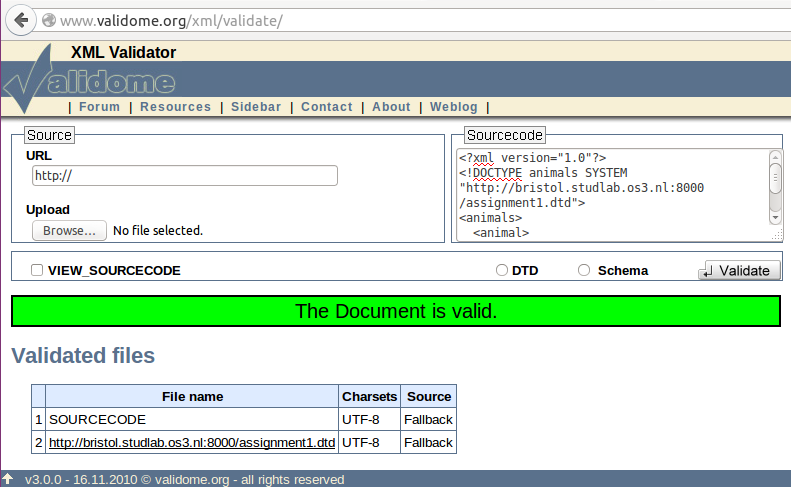
\includegraphics[width=100mm]{img/xmldtdtest.png}
	\caption{Test results of the DTD file}\label{fig:xmldtdtest}
\end{figure}

For the XML schema, I used the schema validator from utilities-online. The proof is to be seen in figure \ref{fig:xmlxsdtest}.

\begin{figure}[h]
	\centering
	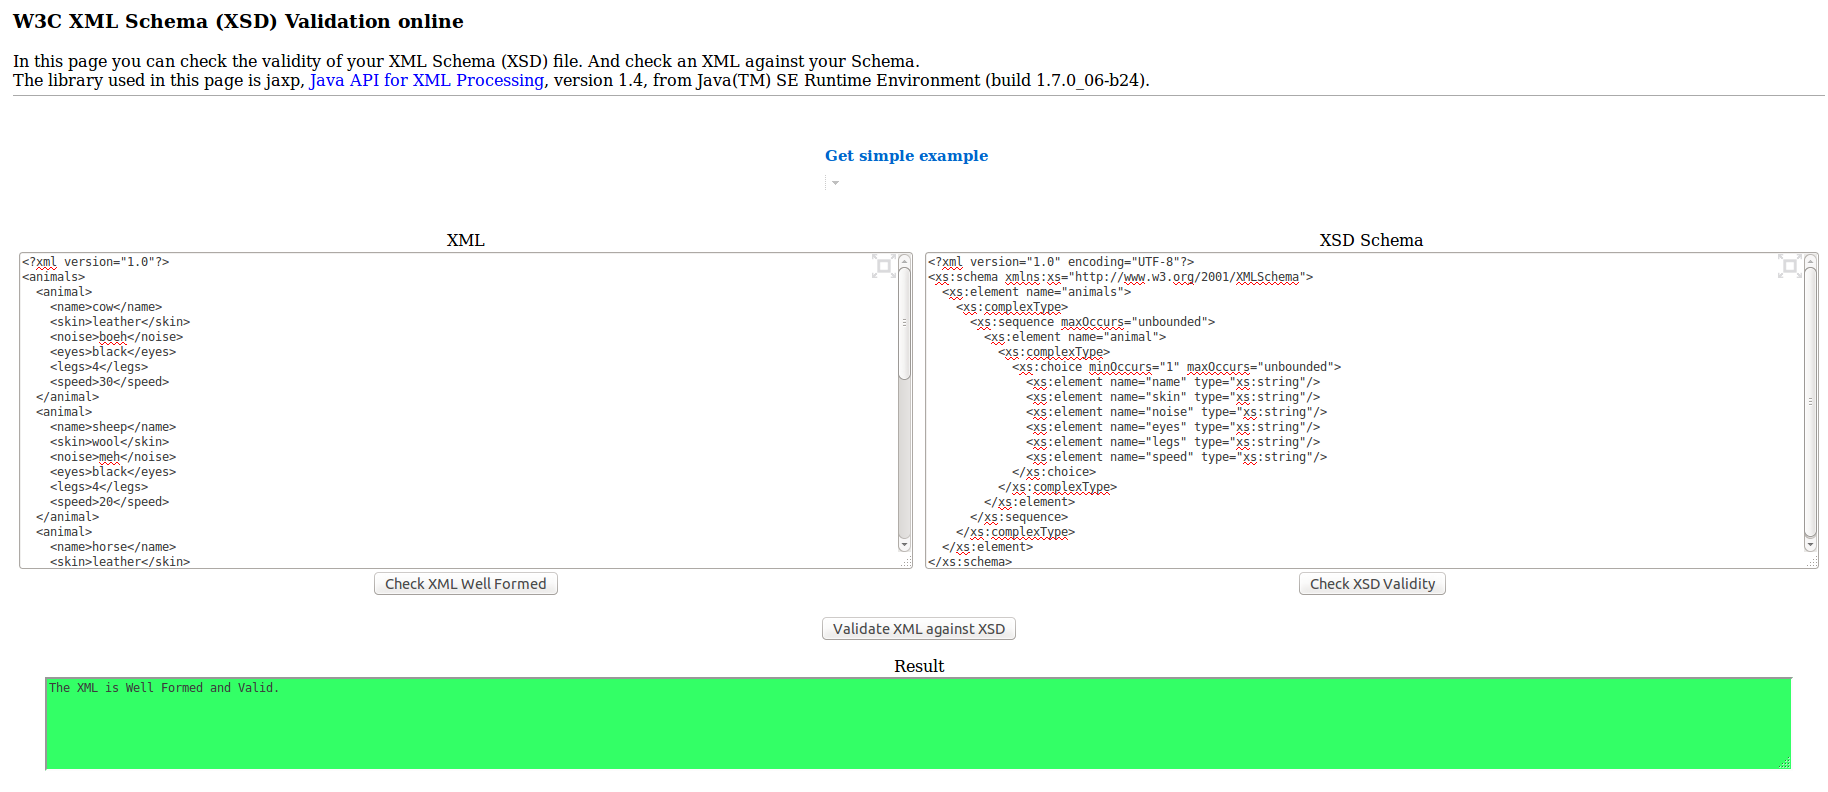
\includegraphics[width=100mm]{img/xmlxsdtest.png}
	\caption{Test results of the XML XSD schema}\label{fig:xmlxsdtest}
\end{figure}

\subsubsection{Assignment 3}
I validated this assignment on w3schools. For the result, check figure \ref{img:xmlxsdtest}.

\begin{figure}[h]
	\centering
	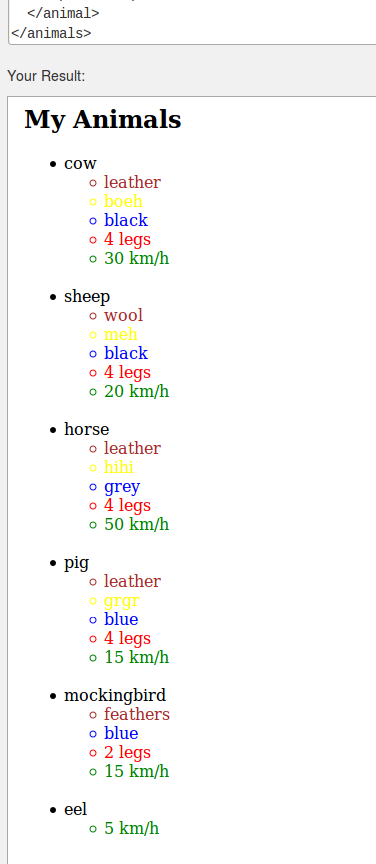
\includegraphics[height=180mm]{img/xhtml.png}
	\caption{Test results of my XHTML and CSS}\label{fig:xhtml}
\end{figure}

\begin{minted}[breaklines]{xml}
<?xml version="1.0" encoding="UTF-8"?>
<xsl:stylesheet version="1.0" xmlns:xsl="http://www.w3.org/1999/XSL/Transform">

<xsl:template match="/">
  <html>
  <head>
  <style type="text/css">
    li.name {
      color: black
    }
    li.noise {
      color: yellow
    }
    li.skin {
      color: brown
    }
    li.eyes {
      color: blue
    }
    li.legs {
      color: red
    }
    li.speed {
      color: green
    }
    li:hover {
      color: grey
    }
  </style>
  </head>
  <body>
  <h2>My Animals</h2>
      <ul>
        <xsl:for-each select="animals/animal">
        <li class="name"><xsl:value-of select="name"/></li>
        <ul>
          <xsl:if test="skin"><li class="skin"><xsl:value-of select="skin"/></li></xsl:if>
          <xsl:if test="noise"><li class="noise"><xsl:value-of select="noise"/></li></xsl:if>
          <xsl:if test="eyes"><li class="eyes"><xsl:value-of select="eyes"/></li></xsl:if>
          <xsl:if test="legs"><li class="legs"><xsl:value-of select="legs"/> legs</li></xsl:if>
          <xsl:if test="speed"><li class="speed"><xsl:value-of select="speed"/> km/h</li></xsl:if>
        </ul>
        <br/>
        </xsl:for-each>
      </ul>
  </body>
  </html>
</xsl:template>
</xsl:stylesheet>
\end{minted}

\subsection{Simple Object Access Protocol}\label{subsection:soap}
SOAP stands for Simple Object Access Protocol, and offers a way for applications to interact with one another. It extensively uses XML to wrap up it's messages. The SOAP standard defines a couple of characteristics. First, every SOAP call is wrapped in an Envelope. Inside the Envelope, a Header may or may not be present. The Header may contain additional information belonging to the request, for example authentication information or preferences. The second element in the Envelope is the Message. This element contains the actual request from the client, or response from the server.

As I wanted to see how a simple SOAP interaction would look like, I created two Python scripts. One sets up an HTTP server and serves a SOAP accessible function. The seconds scripts initiates a client request. The function published by the SOAP server is calculating the square root of a given value.

As to be seen in the code blocks below, the client asks the server to calculate the square root of 9. The server has wrapped it's response to the request in a calculateRootResponse XML element, which contains one sub element. Namely, the outcome of the calculateRoot function. The nice thing to see here, is that the response of the server is treated like a regular Python object. The response.squareRoot contains the response of the server. The scripts were created with the help of the pysimplesoap package.

I found SOAP very easy to use myself. However, the overhead for using SOAP is quite large. According to Wikipedia, financial institutions experienced their message size increased by four times after switching from CDR to SOAP. This can be an argument against using SOAP when trafficking large amounts of data.

\subsection{Experimenting}
As we would like to see how SOAP works, we set up a client-server testapplication in Python. Below is the code for the server.

\begin{minted}{python}
#!/usr/local/bin/python
 
from pysimplesoap.server import SoapDispatcher, SOAPHandler
from BaseHTTPServer import HTTPServer
from math import sqrt
 
def calculateRoot(value):
  return sqrt(value)
 
dispatcher = SoapDispatcher(
    'root_dispatcher',
    location = 'http://localhost:8000/',
    action = 'http://localhost:8000/',
    namespace = 'http://bristol.studlab.os3.nl/root.wsdl', prefix='ns0',
    trace = True,
    ns = True)
 
dispatcher.register_function('calculateRoot', calculateRoot,
    returns = {'squareRoot': float},
    args = { 'value': float })
 
print 'Starting HTTP server'
server = HTTPServer(("", 8000), SOAPHandler)
server.dispatcher = dispatcher
server.serve_forever()
\end{minted}

\paragraph{Client Application}\mbox{}\\
Below is our client application. Pimped with the minted package for \LaTeX.

\begin{minted}{python}
#!/usr/local/bin/python
 
from pysimplesoap.client import SoapClient, SoapFault
 
client = SoapClient(
  location = "http://localhost:8000/",
  action = 'http://localhost:8000/',
  namespace = "http://bristol.studlab.os3.nl/root.wsdl", 
  soap_ns='soap',
  trace = True,
  ns = False)
 
response = client.calculateRoot(value=9)
 
result = response.squareRoot
print float(result)
\end{minted}

\newpage

\section{Buildtools}
Because we are in \textbf{Group 6}, we had to read "Overhauling Amd for the '00s: A Case Study of GNU Autotools" for this weeks homework assignment. Listed below are our remarks regarding the paper. These remarks are split in two pieces; structural remarks which talk about how the paper was structured and substantive remarks which comment on the actual contents of the paper. 

\subsection{Structural remarks}
We found that the paper is well-structured: Zadok starts things of with an explanation about the inner workings of autotools and all its inherent tests and dependencies. After that the writer defines what makes an application difficult to port over to a different system. He concludes with a writeup about how the developers of the ''am-utils'' package benefited from rewriting their ''amd'' package to use autotools (renaming the package to 'am-utils' in the process). The author of the paper lets his own experience weigh in as he has personal experience with autotools which in turn enhances the credibility of his opinions and views.

I do however feel that the conclusion of the paper is a bit lacking. Zadok ends on the notion that autotools helped ''am-utils'' to grow, but also points out a fair amount of weak points in the build tools. Even though he plans on developing a toolkit that can judge how complex a software package is, he does not propose any improvements to the autotools themselves. As he is fairly invested in autotools in general I had hoped to see at least some proposals in regards to making the porting of complex code a more consistent and convenient experience. 

\subsection{Substantive remarks}
Reading the paper is a bit of an emotional rollercoaster. First the author starts out by pointing out all the benefits autotools pose over older methods of building applications. For example, he talks about how the automation factor of the buildtools made it so that end users don't need to have in-and-out knowledge of their system anymore and how code became easier to maintain. Then he all of a sudden starts pointing out the problems autotools have according to him. Although we largely agree with the points he makes throughout the paper, we question some of his partial conclusions. To illustrate we'll go over some of these partial conclusions and note our remarks below. 

At some point in the paper Zadok talks about how the tests in autotools are very extensive, but don't cover all the needs of developers. He writes the following:

\begin{quotation}
"The conclusion we draw in this section is that although Autoconf continues to evolve and provide more tests, maintainers of large and complex packages may still have to write 10–30 custom macros. Moreover, some packages will always need a number of static macros, for those features that Autoconf cannot test in a reliable, automated way".
\end{quotation}

As a reader I feel that it is unfair to fault autotools for this 'problem' too much, because this was a problem initially as well. Before autotools were introduced developers and administrators had to jump convoluted hoops in order to port their application to different platforms. Granted, it is supposedly difficult to convert a package to use autotools, but it (should be) worth it in the end as the buildtools make the need for custom macros a lot lower. Because Autoconf out of the box supports a whole slew of pre-created tests, the developers of ''am-utils'' only had to write new tests for a small portion of their code. Table \ref{table:worthlesstable} shows a pretty worthless table.

\begin{table}[H]
	\center
	\begin{tabular}{|c|c|c|}
	\hline 
	\textbf{Amount of lines} & \textbf{C++ constructs} & \textbf{System calls} \\ 
	\hline 
	Bad & Good & Best \\ 
	\hline 
	\end{tabular}
	\caption{This is a worthless table}
	\label{table:worthlesstable}
\end{table}

A substantial part of the paper talks about the complexity of code and the different metrics used to measure this complexity. Even though I am not a software developer I disagree to some extent with the metrics for code complexity posed in the paper. In the first graphs, the number of lines of code is used as a complexity metric. Luckily the writer also takes up other metrics in the latter part of the report. Zadok settles on the metric of the ''amount of CPP constructs per 1000 lines of code''. Although this lets you know something about the overall complexity of the code it is in my opinion unrelated to the portability issues which the author encountered whilst incorporating autotools in ''amd''. 

Namely, the amount of low level system calls which the package has to make made porting the application so difficult. ''am-utils'' makes use of a lot of lowlevel kernel calls which in turn require a lot of custom or static Autoconf tests. The portability of the application is therefore closely related to the amount of system calls an application makes. Even though software like ''gcc'' and ''Binutils'' are much larger applications, they mainly do text-parsing, which usually consists of rather portable code. Even though the code that the application is written in is generally cross-platform, the system calls that the program makes are non-standardized which naturally creates code portability issues. Therefor I think the ''amount of system calls per 1000 lines of code'' defines the complexity for portability better. I may be mistaken, but I feel the writer is talking about different kinds of complexity throughout his paper. 

\begin{quotation}
"The conclusion we draw from our experiences is that large packages can benefit greatly from using autotools such as Autoconf. Autoconf-based packages are easier to maintain, develop, and port to new systems".
\end{quotation}

Even though this statement holds true in most cases, Zadok also states that their ''amd'' package grew in functionality (which took around 60.000 lines of code) after the incorporation of autotools. Therefor I personally think that not only large packages can benefit from autotools as smaller packages could benefit from the enhanced code maintaining functionality as well. They would get the chance to grow faster due to the incorporation of the build tools. 

Lastly, the paper mentions that compiling code with autotools is five times slower than directly building the package due to the different steps the autotools have to take in order to compile a package. It is questionable whether this is still a problem in modern day and age due to the increased speed of processors. Mind you that the tests performed in that paper make use of a \textit{Pentium III processor} with 128MB of RAM. Personally I think that the speed gain from \underline{not} using autotools nowadays is negligible. 

\begin{figure}[H]
	\centering
	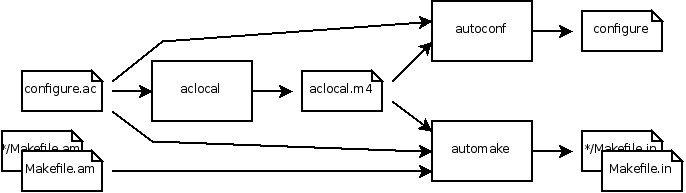
\includegraphics[scale=0.4]{./img/autotools.png}
	\caption{A totally pointless image}
	\label{fig:pointlessimage}
\end{figure}

Judging from my current knowledge about the subject, I think that autotools have been good for development, and I think it would be hard to argue against that. Zadok encountered that the conversion from ''amd'' to ''am-utils'' was a rather bumpy ride. However, I think that this was largely due to the fact that he tried to incorporate autotooling in the original ''amd'' package. Perhaps if a developer would create an application right now and would incorporate the autotools from the beginning, the overall experience would be a lot smoother. Furthermore, as Zadok states in his paper, ''am-utils'' is unique in the sense that the package requires a large amount of low-level system calls which makes the package portability inherently much more difficult. Also take a look at figure \ref{fig:pointlessimage} below \footnote{Using Autotools. (n.d.). Retrieved September 27, 2015, from https://developer.gnome.org/anjuta-build-tutorial/stable/create-autotools.html.en}.

\subsection{Closing remarks}
We generally agreed on the points posed in the text above. Below are however some extra points points about the paper. 

\emph{\textcolor{red}{Bram ter Borch}}
\begin{quotation}
"In my opinion the paper was fine to read. But it was very detailed in the way he had to work around the shortcomings in the auto tools for his specific application. The examples of his own test scripts do not add anything to the paper. Beside that he introduces a new way to measure complexity. So you are right, he is talking about different ways of complexity."
\end{quotation}
\textit{Bram also writes the following:}

\begin{quotation}
In your document, you write about the speed of compiling. I think it didn't change over time. Zadok is right about his statement. He tested compiling and installing the application before auto tooling and after. When compiling auto tools needs to do a lot of checks. This takes time. And nowadays programs become much larger than 10 years ago. Auto tools contains a lot more tests it needs to work through. Due to the increase of operating systems in my opinion compiling a program is not a lot faster than 10 years ago. Even with the hardware we currently have.
After a short discussion we have agreed to disagree on this point. I personally hold the opinion that the amount of tests hasn't had the same turbulent growth that processors have had. I may however be wrong on this. 

I share you opinion in the advantage of auto tools. It is the way to go. Zadok took a long time to master auto tools, he needed to change his way of programming to fit into the auto tools ways, but in the long run he, and the functionality of the package greatly benefit from the incorporation.
\end{quotation}

\emph{\textcolor{red}{Jeroen Schutrup}}
\begin{quotation}
"I agree with both of you guys arguments. Something that was not clear to me was the fact that am-utils was more complex than amd after they moved to autotools, to be seen in Figure 3. Besides, I wonder how much of a burden the complexity overhead of not having autotools actually was. After they switched to autotools, their codebase decreased from 90k to 60k lines. From there on, they managed to recreate these 30k lines of code they've just saved, almost within one month worth of time. So I wonder how much of an issue the complexity was to them."

With this notion Jeroen highlight the biggest problem I have with this paper: the concept of complexity is very loosely defined throughout the paper. The increase in code however was due to the added functionality. This functionality could be added because it became easier to maintain the codebase after autotools were introduced in the build process. 
\end{quotation}

\newpage
\section{Regex Engines}
Group 4, 5 and 6 need to explain what the difference is about text-directed and regex-directed engine for regex.
source : http://www.regular-expressions.info/engine.html

\subsection{technologies}
There are two underlying technologies commonly used to implement a regex match 
engine: regex-directed NFA (Nondeterministic Finite Automation) and 
text-directed DFA (Deterministic Finite Automation). Of the two types of 
engines, “NFA” is more commonly used. Popular programming languages like Python, Ruby 
and PHP use the formatting provided by NFA engines. DFA engines are more commonly seen 
in tools like egrep and awk. grep even employs a hybrid engine model where situationally 
the type of engine is switched around.

\subsection{matching}
A NFA must try every possible permutation of the regex before it can conclude that there's 
no match. A DFA finds the longest leftmost match. A Traditional NFA might also, or it might find something 
else. Any individual engine always treats the same regex/text combination in the 
same way, so in that sense, the regex isn't random, but other NFA engines may 
decide to do slightly different things. DFA Text-Directed Engines find the longest 
possible match. They are considered to be consistent and very fast due to their 
ability to simultaneously parse portions of the regex. NFA Regex-Directed Engines 
must work through a match. An NFA engine can support many things that a DFA cannot. 

Basically the regex-directed engine is way more flexible.
It contain options like:
\begin{itemize}
  \item lazy quantifiers (backtratracking of options) ex: \begin{verbatim}<.+?>\end{verbatim}
  \item backreferences (Matches the same text as matched previously)
  \item atomic grouping (based to a capturing group but without backtracking) ex: \begin{verbatim}a(?>bc|b)c\end{verbatim}
  \item possessive quantifiers (prevent the engine from trying all permutations)
\end{itemize}

During the course of an NFA match, the same character of the target 
might be checked by many different parts of the regex (or even by the same part, 
over and over). Even if a subexpression can match, it might have to be applied again 
(and again and again) as it works in concert with the rest of the regex to find a match. 
A local subexpression can fail or match, but you just never know about the overall match 
until you eventually work your way to the end of the regex. On the other hand, a DFA 
engine is deterministic: each character in the target is checked once (at most). When a 
character matches, you don't know yet if it will be part of the final match (it could be 
part of a possible match that doesn't pan out), but since the engine keeps track of all 
possible matches in parallel, it needs to be checked only once, period.

\begin{figure}[h]
	\centering
	
\includegraphics[width=100mm]{img/regex.png}
	\caption{I know Regex}
\end{figure}

\newpage
\printbibliography{}							% Print the bibliograpy => page with external sources/references
\newpage
\mbox{}\newpage
\begin{appendices}							% Special section for appendices. Every appendice is stored in its own tex file
	\section{XML DTD Source}\label{appendice:xmldtdsrc}
\begin{minted}{XML}
<?xml version="1.0"?>
<!DOCTYPE animals SYSTEM "http://bristol.studlab.os3.nl:8000/assignment1.dtd">
<animals>
  <animal>
    <name>cow</name>
    <skin>leather</skin>
    <noise>boeh</noise>
    <eyes>black</eyes>
    <legs>4</legs>
    <speed>30</speed>
  </animal>
  <animal>
    <name>sheep</name>
    <skin>wool</skin>
    <noise>meh</noise>
    <eyes>black</eyes>
    <legs>4</legs>
    <speed>20</speed>
  </animal>
  <animal>
    <name>horse</name>
    <skin>leather</skin>
    <noise>hihi</noise>
    <eyes>grey</eyes>
    <legs>4</legs>
    <speed>50</speed>
  </animal> 
  <animal>
    <name>pig</name>
    <skin>leather</skin>
    <noise>grgr</noise>
    <eyes>blue</eyes>
    <legs>4</legs>
    <speed>15</speed>
  </animal> 
  <animal>
    <name>mockingbird</name>
    <skin>feathers</skin>
    <eyes>blue</eyes>
    <legs>2</legs>
    <speed>15</speed>
  </animal>
  <animal>
    <name>eel</name>
    <speed>5</speed>
  </animal> 
</animals>
\end{minted}

	\newpage
\end{appendices}
\end{document}
